\documentclass[11pt]{article}
\ifdefined\XeTeXrevision\else\pdfoutput=1\fi

\usepackage[
  left=0.85in,
  right=0.85in,
  top=0.80in,
  bottom=0.75in,
  footskip=0.35in
]{geometry}
\usepackage{amsmath,amssymb,amsthm,bm}
\usepackage{graphicx}
\usepackage{booktabs}
\usepackage{float}
\usepackage{microtype}
\usepackage{caption}
\usepackage{titlesec}
\captionsetup{font=small,skip=9pt,justification=raggedright,singlelinecheck=false}
\captionsetup[table]{position=above}
% Shared math macros for the paper. Kept small and self-contained.
% (Packages are loaded in main.tex so that hyperref can be loaded last.)

% --- objects -----------------------------------------------------------------
\newcommand{\R}{\mathbb{R}}
\newcommand{\mat}[1]{\bm{#1}}                 % a matrix / block
\newcommand{\inv}[1]{#1^{-1}}
\newcommand{\T}{^{\mathsf{T}}}                % transpose
\newcommand{\selinv}{\operatorname{SelInv}}  % selected inverse on the pattern
\newcommand{\pat}{\mathcal{S}}               % the (filled) sparsity pattern
\newcommand{\Gr}{\mathcal{G}}                % the graph
\newcommand{\diagop}{\operatorname{diag}}
\newcommand{\trace}{\operatorname{tr}}
\newcommand{\bigO}{\mathcal{O}}
\newcommand{\loss}{\mathcal{L}}

% --- selected blocks / factors ----------------------------------------------
\newcommand{\Gblock}[2]{G_{#1#2}}            % a block of A^{-1}
\newcommand{\Ablock}[2]{A_{#1#2}}
\newcommand{\piv}[1]{D_{#1}}                 % pivot block
\newcommand{\fac}[1]{\ell_{#1}}             % factor block ell_v = A_{p,v} D_v^{-1}

% --- adjoints (cotangents): \cotan{G} = \partial f / \partial G ---------------
% (named \cotan because \cot is the LaTeX cotangent operator)
\newcommand{\cotan}[1]{\bar{#1}}

\newcommand{\children}{\operatorname{ch}}
\newcommand{\parent}{p}

\usepackage[colorlinks=true,linkcolor=blue,citecolor=blue,urlcolor=blue]{hyperref}
\hypersetup{
  pdftitle={Exact Sparse Operators in Differentiable Models:
            Attainability, Not Inductive Bias},
  pdfauthor={Vanshdeep Sehrawat},
}

\setlength{\emergencystretch}{1em}
\linespread{1.25}

% The body uses named paragraph-level arguments, but run-in headings make the
% manuscript visually dense. Set them as short display headings instead.
\titleformat{\paragraph}[block]
  {\normalfont\normalsize\bfseries}{}{0pt}{}
\titlespacing*{\paragraph}{0pt}{1.15\baselineskip}{0.35\baselineskip}

\raggedbottom

\theoremstyle{plain}
\newtheorem{theorem}{Theorem}
\newtheorem{lemma}{Lemma}
\newtheorem{corollary}{Corollary}
\theoremstyle{remark}
\newtheorem{remark}{Remark}

\begin{document}

\begin{titlepage}
\renewcommand{\thefootnote}{\fnsymbol{footnote}}
\begin{center}
\vspace*{0.2cm}

{\LARGE Exact Sparse Operators in Differentiable Models:\\[0.45em]
Attainability, Not Inductive Bias\par}

\vspace{0.9cm}

{\large Vanshdeep Sehrawat\footnote{e-mail:
  \texttt{sehrawat@unlv.nevada.edu}, \texttt{vanshdeep.sehrawat@gmail.com};\ ORCID:
  \href{https://orcid.org/0009-0005-8062-1337}{0009-0005-8062-1337}.}}\\[0.35em]
{\itshape University of Nevada, Las Vegas, USA}\\[0.35em]
{\small July 2026}

\vspace{0.9em}

{\small Code, data, and frozen pre-registration records:
\href{https://github.com/vanshsehrawat14/gabp-sparse-inv}{\texttt{github.com/vanshsehrawat14/gabp-sparse-inv}}
(package \texttt{gabp-sparse-inv} on PyPI).\\
File paths cited in this paper are relative to the repository root.}

\vspace{0.45cm}

{\bfseries Abstract}
\end{center}

\begin{quote}\small
Many machine-learning models require a global linear solve. For sparse,
fixed-width coupling, selected inversion computes inverse blocks on the
factor's filled pattern in $\bigO(n)$ time, and its projected derivative has
a reverse schedule with the same asymptotic structural work. We implement
the classical symmetric and static-pattern non-symmetric operators as
differentiable PyTorch primitives. The scientific question is whether an
exact structured solve acts as an \emph{inductive bias}, selecting a
better-generalizing solution when competing models attain comparable
training fit. Two pre-registered matched-fit probes test this hypothesis on
$30$ held-out seeds: routed-field size extrapolation and deep-equilibrium
training near spectral instability. The exact arms win the raw comparisons,
but the finite Jacobi and Neumann alternatives match their training fit in
only $0$--$23\%$ of high-difficulty seeds, below a pre-registered $60\%$
bar. The equal-fit comparison is therefore absent; under the tested budgets,
the result is an \emph{attainability/optimization} gap, not an
inductive-bias effect. In separate diagnostics, the exact routed-field model
beats larger GNN and Transformer baselines by roughly $600\times$ in
distribution and up to $28{,}000\times$ under extrapolation. The
sparse-direct implicit backward remains within $1.1\times10^{-12}$ of a
dense fp64 oracle on four stiffness cells where finite Neumann adjoints are
$77$--$100\%$ wrong at $\rho(J)\in\{0.99,0.999\}$; an fp32 sweep finds no
robust precision advantage over a well-ordered dense factorization. The
DEQ low-difficulty control fails its pre-specified relative-gap clause, and
two non-equivalent maze-floor diagnostics disagree. A later reuse of the
same held-out seeds is excluded. The supported conclusion is therefore
narrow and hedged: exact structured computation expands the attainable
regime in these controlled, solve-shaped CPU probes, while the proposed
inductive-bias explanation is not supported.
\end{quote}

\end{titlepage}
\setcounter{page}{2}

\section{Introduction}
\label{sec:intro}

Anywhere a model relies on self-consistency, soft constraint satisfaction, or a
fixed point, it pays for a matrix inverse. Deep equilibrium models
differentiate through an equilibrium with the implicit function theorem
\cite{bai2019deep}; linear-attention and delta-rule layers mix tokens with a
triangular solve \cite{yang2024parallelizing}; implicit and steady-state graph
layers solve for a fixed point. In each case the forward pass, and almost
always the backward pass, is a linear solve. The general inverse is
$\bigO(n^3)$. When the coupling is sparse on a low-treewidth graph, the
\emph{selected} inverse, meaning only the blocks of $\inv{A}$ on the factor's
filled sparsity pattern, is computable in $\bigO(n)$ on fixed-width families
and $\bigO(n^{1.5})$ on 2-D
grids via Gaussian belief propagation and the Takahashi recurrence
\cite{takahashi1973,erismantinney1975}, never forming the dense inverse.
Recent selected-inversion and differentiable-sparse-solver systems establish
that this is an active implementation area
\cite{maillou2025serinv,fattah2025stiles,wang2025schwarz,torchsla2026};
the present paper does not claim a new forward algorithm or a performance
record.

\paragraph{Research question.}
Sparse direct computation removes iteration truncation, but it does not imply
greater floating-point accuracy. On the finite precision grid in
Section~\ref{sec:numerics}, selected inversion and a well-ordered dense solve
perform comparably when scored on the selected pattern against an fp64
oracle. The question examined here is instead:
\begin{quote}
\emph{When does the exactness of a structured linear-algebra primitive change
what a neural network can learn or generalize, as opposed to merely how fast
or how accurately it computes a fixed quantity?}
\end{quote}

\paragraph{Hypothesis and adjudicated outcome.}
The hypothesis was that an exact, size-agnostic global solve supplies an
inductive bias: among models with comparable training fit, it selects a
solution that generalizes better. Two pre-registered probes test this on
$30$ held-out seeds with matched-fit rules
(\url{archive/docs/CONFIRMATORY_RESULTS.md}). In the high-difficulty cells,
the finite alternatives match the exact arm's training fit in only
$0$--$23\%$ of seeds, below the pre-registered $60\%$ bar. The equal-fit
comparison required by the hypothesis does not arise. The first-read
evidence therefore supports an attainability/optimization interpretation,
not an inductive-bias effect.
\begin{itemize}
  \item \emph{Size extrapolation.} A $65$-parameter model containing the
        exact solve remains accurate as the routed-field grid grows, while
        larger GNN and Transformer baselines approach the predict-the-mean
        floor. Replacing only the solve with $K$ Jacobi sweeps produces a
        monotone reach-dependent gap, but none of the tested truncations
        attains the exact arm's training fit (Section~\ref{sec:maze}).
  \item \emph{Stiff-regime training.} On four diagnostic cells, the
        sparse-direct implicit backward agrees with a dense fp64 oracle to
        within $1.1\times10^{-12}$, whereas finite Neumann adjoints degrade
        as $\rho(J)$ approaches one. In the pre-registered training study,
        the iterative-adjoint arm does not attain comparable fit in the
        stiff cells (Section~\ref{sec:deq}).
\end{itemize}
The DEQ low-difficulty control fails its relative-gap clause. The maze
extrapolation-floor comparison passes, but a separate in-distribution
\texttt{floor\_sound} diagnostic is false. The paper retains both limitations.

\paragraph{Contribution.}
The exact forward engine is classical
\cite{takahashi1973,erismantinney1975,lin2011selinv,weiss2001correctness}.
That its differentiable reverse schedule has forward-order structural work
is also not new: selected inversion is the projected gradient of a log-determinant
\cite{zhu2019sparse,dwyer1948symbolic}, so reverse mode costs a constant
multiple of the forward \cite{baur1983complexity}. Both are stated once, as
mathematical background (Section~\ref{sec:theorem}). The contributions are:
\begin{enumerate}
  \item an integrated PyTorch operator family for differentiable selected
        inversion and its solve siblings;
  \item two pre-registered matched-fit studies that distinguish an
        equal-fit preference from a failure to attain comparable training
        fit; and
  \item a boundary analysis separating the measured result from claims that
        require stronger solver baselines and new protocols
        (Section~\ref{sec:program}).
\end{enumerate}

\paragraph{Scope.}
The present evidence is at controlled, CPU scale: routing grids up to
$10\times10$ for the baseline comparison and up to $48\times48$ for the
held-out matched-compute control, and deep-equilibrium fixed points at
$n\le16$. The structural win is confined
to low-treewidth (1-D and quasi-2-D) problems; general 3-D problems have
prohibitive frontal growth for the claimed direct regime. The benchmark-scale
questions in Section~\ref{sec:program} require
separate protocols, mature sparse-direct backends, and matched accuracy/cost
comparisons; they are not evidence in this paper.

\section{The primitive: an exact, differentiable global sparse solve}
\label{sec:primitive}

The vehicle for the operator family under test is a differentiable selected-inverse layer.
The later sections need three facts about it: it is exact and global
(\S\ref{sec:setup}), it is differentiable at the asymptotic cost of its
forward pass (\S\ref{sec:theorem}), and it is available across the matrix
structures the experiments use (\S\ref{sec:kernels}). None of the three is
new. Together they make exactness embeddable and trainable.

\subsection{Selected inversion on a pattern}
\label{sec:setup}

Let $A \in \R^{N\times N}$ be a block matrix with $n$ diagonal blocks of size
$b$ ($N = nb$) whose block sparsity pattern is a graph $\Gr$ on the $n$ nodes.
The \emph{selected inverse} on a pattern $\pat \supseteq \Gr$ is
\begin{equation}
  \selinv_{\pat}(A) \;=\; \{\, \Gblock{u}{v} \;:\; (u,v)\in\pat \,\},
  \qquad \Gblock{u}{v} = \big(\inv{A}\big)_{uv},
  \label{eq:selinv-def}
\end{equation}
that is, the blocks of $\inv{A}$ on $\pat$ only, never the dense inverse. For
SPD $A$ the natural pattern is the pattern of $A$ itself when $\Gr$ is a tree
(zero fill), and the filled (chordal) pattern
$\pat = \mathrm{pattern}(L+L\T)$ otherwise. Most entries of $\inv{A}$ are dense
and cannot even be materialized at scale; the on-pattern blocks are exactly
what marginal-variance and log-determinant-gradient computations read.  The
same sparse factors also supply the solve siblings used for routed fields
$\inv{A}e_s$ and fixed-point backwards.

\paragraph{Why it is global, exact, and structurally sparse.}
$\inv{A}$ couples every node to every other: $\Gblock{u}{v}$ is a global
functional of the whole graph, not of a local neighbourhood. Yet if $\Gr$ has
low treewidth, a fill-reducing elimination order keeps the elimination fronts
small. More precisely, let $U_v$ be the later neighbours of node $v$ in the
filled graph, and define
\[
  F=\sum_v(1+|U_v|),\qquad W=\sum_v(1+|U_v|^2).
\]
$F$ counts factor-pattern blocks, whereas $W$ counts dense clique work.
Numeric storage is $\Theta(Fb^2)$ and factorization plus selected inversion is
$\Theta(Wb^3)$. They are proportional at bounded treewidth, but not in
general: both are $\Theta(n)$ on trees, while nested dissection on a 2-D grid
has $F=\Theta(n\log n)$ and $W=\Theta(n^{3/2})$. The Takahashi recurrence
computes \eqref{eq:selinv-def} algebraically exactly, up to floating-point
rounding, rather than by a convergence-truncated iteration. Its work depends
on elimination structure, not on the number of message-passing iterations
needed to traverse the graph.

\paragraph{The target regime.}
The target is well-scaled operators with large condition number, e.g.\
graph-Laplacian precisions $A = L(W) + \varepsilon I$ with $\bigO(1)$ entries
and $\kappa \approx \lambda_{\max}/\varepsilon$. SPD Cholesky needs no
pivoting, but its forward accuracy remains condition-sensitive; ``direct''
means iteration-independent, not condition-independent. The non-symmetric
kernel additionally assumes a static no-pivot pattern and nonsingular Schur
pivots. These restrictions are material when the coupling is long-range.

\subsection{Why it is differentiable at forward cost}
\label{sec:theorem}

For the layer to be usable as a learned component it must be trainable. That it is,
at no asymptotic overhead, is a classical fact, stated once and built on.

\begin{remark}[Selected inversion is a gradient; its derivative has a sparse reverse schedule]
\label{rem:scaffold}
Write $P_{\pat}$ for orthogonal projection onto the on-pattern blocks. Under
the full Frobenius inner product on the symmetric matrix subspace, selected
inversion is the on-pattern gradient of the log-determinant,
$\selinv_{\pat}(A)=P_{\pat}\nabla_A\log\det A$
\citep{zhu2019sparse,dwyer1948symbolic}. Its derivative is therefore
self-adjoint after projection to that subspace. Reverse mode can be evaluated
by reversing the same elimination and Takahashi primitives, with no denser
pattern. By the cheap-gradient principle \citep{baur1983complexity}, its
arithmetic cost is a constant multiple of the forward's
$\Theta(Wb^3)$ work; the analytic implementation stores the factors and
selected blocks rather than an operation-by-operation autograd tape. For
non-symmetric $A$, write
$L_A:X\mapsto-\inv{A}X\inv{A}$ for the inversion derivative. Its adjoint is
$L_{A\T}$, not a selected inverse by itself. This transposes the
factor roles and requires independent lower and upper cotangents. The tree
specialization and projected-adjoint statement are in
Appendix~\ref{app:theorem}.
\end{remark}

Remark~\ref{rem:scaffold} is why the exact, global sparse solve of
\S\ref{sec:setup} can be used as a layer: embedded in a model and trained
end-to-end with the same asymptotic structural work as the forward pass, never forming the dense
inverse. From here the question is what the exactness of this layer does to
learning.

\subsection{Implemented operator family}
\label{sec:kernels}

The operator must be available wherever the experiments need it, so the package ships the
selected inverse and its adjoint as drop-in PyTorch operators across a small
generality ladder (Table~\ref{tab:ladder}). The symmetric rung covers the
block chain (the Rauch--Tung--Striebel / Kalman-smoother form
\cite{rauch1965maximum}), the star, the
general tree, and, via a symbolic elimination that completes the pattern to
the chordal $\pat = \mathrm{pattern}(L+L\T)$, the general sparse SPD
junction-tree case. The non-symmetric rung runs from the triangular chunk
inverse $(I-A)^{-1}$ (the delta-rule primitive) through the zero-fill
non-symmetric tree to the general filled-pattern LU (Erisman--Tinney) selected
inverse, whose inversion derivative is adjoint up to transpose
(Remark~\ref{rem:scaffold}). Every operator family is checked against a dense
oracle on its documented test grid. Differentiable kernels are validated by \texttt{gradcheck}; the
functional kernels that support higher-order autograd are additionally checked
by \texttt{gradgradcheck}. The filled-pattern kernels also ship hand-written
tape-free analytic backwards whose autograd graphs are constant-size regardless
of $n$; these analytic backwards are first-order operators and are validated
against the functional paths. The engineering boundary (no pivoting; the
static-pattern regime) is described in
Appendix~\ref{app:engine}.

\begin{table}[H]
  \centering
  \caption{Implemented selected-inverse operators. The forward recurrences are
  classical; the differentiable adjoints make them trainable. For the
  non-symmetric rows, $L_A^*=L_{A\T}$ denotes the inversion derivative, not
  the selected-inverse value at $A\T$.}
  \label{tab:ladder}
  \begin{tabular}{lll}
    \toprule
    Structure & Forward (classical) & Differentiable adjoint \\
    \midrule
    Chain / star / tree (SPD)        & GaBP / Takahashi, zero fill        & self-adjoint, $\bigO(n)$ \\
    Junction tree (general SPD)      & Takahashi on chordal $\pat$        & projected derivative self-adjoint \\
    Triangular $(I-A)^{-1}$          & delta-rule chunk solve             & self-adjoint up to transpose \\
    Non-symmetric tree / LU          & Erisman--Tinney on $\pat$          & self-adjoint up to transpose \\
    \bottomrule
  \end{tabular}
\end{table}

\section{Exactness is not accuracy}
\label{sec:numerics}

Before attributing the learning probes to operator structure, the paper checks
whether this implementation has a floating-point accuracy advantage.
It does not on the finite precision grid below. The grid supplies no evidence
for that explanation; it is not a universal comparison of
sparse and dense factorization accuracy.

\paragraph{No robust win in either direction.}
Scored on the pattern against a 64-bit oracle and swept over conditioning
(Table~\ref{tab:precision}), the selected inverse and a dense SPD solve at
equal 32-bit floating-point (fp32) precision stay within small constant
factors of each other across
structures and $\kappa$: the error ratio ranges from $0.34$ to $1.95$ with no
consistent direction (at the highest-$\kappa$ grid cell the dense solve is in
fact the more accurate, by more than $2.8\times$). An initial reading of roughly $1.9\times$
on trees, growing with $\kappa$, on ill-scaled random matrices turned out,
over enough seeds (16 for the ordering study), to be a ratio-of-medians
artifact, and most of the modest, heavy-tailed median gap is an
elimination-ordering effect: a dense Cholesky run in the kernel's own
leaf-first order has comparable accuracy. No consistent accuracy edge appears
on this grid. The 16-seed ordering diagnostic is recorded in
\url{paper/attainability/figures/data/precision_compare_orders.txt}.

\begin{table}[htbp]
  \centering
  \caption{Selected inverse vs.\ dense Cholesky at equal fp32 precision,
  scored on-pattern against an fp64 oracle. Entries are medians over four
  seeds per cell; the ratio is the median per-seed dense/selected-inverse
  error ratio. Displayed errors and ratios are rounded conservatively against
  the selected-inverse arm. Data:
  \url{paper/attainability/figures/data/precision_tree.csv} and
  \url{paper/attainability/figures/data/precision_grid.csv}.}
  \label{tab:precision}
  \begin{tabular}{lcccc}
    \toprule
    structure & $\kappa$ & selected-inverse error & dense error & ratio \\
    \midrule
    tree ($n{=}127$) & $6.0\mathrm{e}{+1}$ & $1.6\mathrm{e}{-7}$ & $2.0\mathrm{e}{-7}$ & $1.32$ \\
    tree ($n{=}127$) & $5.8\mathrm{e}{+3}$ & $6.2\mathrm{e}{-6}$ & $1.1\mathrm{e}{-5}$ & $1.95$ \\
    tree ($n{=}127$) & $2.9\mathrm{e}{+5}$ & $4.2\mathrm{e}{-4}$ & $4.5\mathrm{e}{-4}$ & $1.64$ \\
    grid ($8{\times}8$) & $1.8\mathrm{e}{+1}$ & $1.7\mathrm{e}{-7}$ & $1.4\mathrm{e}{-7}$ & $0.88$ \\
    grid ($8{\times}8$) & $1.7\mathrm{e}{+3}$ & $3.2\mathrm{e}{-6}$ & $3.4\mathrm{e}{-6}$ & $1.10$ \\
    grid ($8{\times}8$) & $1.7\mathrm{e}{+5}$ & $8.5\mathrm{e}{-4}$ & $2.7\mathrm{e}{-4}$ & $0.34$ \\
    \bottomrule
  \end{tabular}
\end{table}

\paragraph{What exactness does give: a sparse-structured global operator.}
The edge is not a more accurate rounded number; it is that the operator is
algebraically exact, global, and sparse-structured. That structure is what
makes the operator usable as a layer:
Figure~\ref{fig:scaling} shows forward timings consistent with the chain's
$\bigO(n)$ operation count, with the measured dense crossover, and
forward-plus-backward Gaussian Markov random field (GMRF) training timings
consistent with linear tree work
where dense autograd is $\bigO(N^3)$. The cost still grows with problem size,
linearly on the chain shown here; it does not acquire an iteration count
proportional to graph distance. That is the distinction the next two sections
exploit.

\providecommand{\scalingfigurewidth}{0.92\textwidth}
\begin{figure}[htbp]
  \centering
  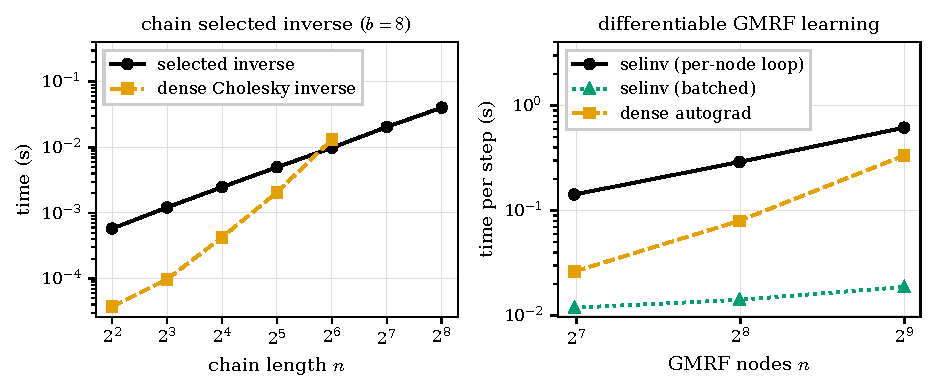
\includegraphics[width=\scalingfigurewidth]{figures/scaling.pdf}
  \caption{Scaling diagnostics on a central processing unit (CPU). Left:
  forward time for a 64-bit floating-point (fp64) block-chain
  selected inverse ($b=8$) and a dense Cholesky inverse, using the median of
  three seed-wise timing medians. Right: forward-plus-backward time per
  differentiable tree Gaussian Markov random field (GMRF) training step and
  dense autograd. Timings depend on the basic linear algebra subprograms
  (BLAS) library and device; no graphics processing unit (GPU) claim is made.
  Data:
  \href{bench_results.csv}{\texttt{bench\_results.csv}}
  and
  \href{paper/attainability/figures/data/gmrf_scaling.csv}{\texttt{gmrf\_scaling.csv}}.}
  \label{fig:scaling}
\end{figure}

\section{Probe 1: size extrapolation with an exact structured solve}
\label{sec:maze}

If exactness is an inductive bias for solve-shaped tasks, its cleanest
signature is size generalization: a model whose global computation is exact at
every size, and whose parameters do not depend on size, should keep working as
the problem grows, while a learner that must approximate the global
computation from finite data should not. A routing task tests this; a
within-architecture control then isolates the cause.

\paragraph{Task and models.}
Each example is a random grid-Laplacian precision $A = L(w) + \varepsilon I$
and a source $s$; the label is the routed field $\inv{A}\,e_s$, an exact,
global functional of the whole graph. A \texttt{gabp} model consumes strictly
local per-node inputs $[\phi_v, \deg_v, b_v]$. Its small ($65$-parameter,
size-independent) pointwise encoder maps $[\phi_v,\deg_v]$ to an SPD
precision, while $b_v$ is the solve right-hand side; the model then applies
one differentiable factorization layer. Two baselines consume the same local
inputs: a deep residual message-passing GNN ($22\,337$ parameters,
$343\times$ the trainable-parameter count)
and a full-attention Transformer with 2-D sinusoidal positions ($18\,305$
parameters, $281\times$ the count; global reach at every layer). Positive node
potentials produced by \texttt{softplus} keep the induced edge weights
positive, and the $\varepsilon I$ lift removes the Laplacian nullspace. This
guarantees SPD input but does not fix the condition number.

\paragraph{Size-extrapolation result.}
Trained at $6\times6$ and evaluated up to $10\times10$ (Table~\ref{tab:maze},
Figure~\ref{fig:maze}), the displayed \texttt{gabp} median stays below
$10^{-4}$ at every size while both baselines move toward the predict-the-mean
floor as the diameter grows; the three-seed ranges in the recorded CSV do not
overlap. The
displayed median error ratios are $212\times$--$903\times$ at the training
size and $9{,}448\times$--$11{,}242\times$ at $10\times10$. These are
diagnostic comparisons, not lower bounds on what other GNN or Transformer
architectures could attain.

\begin{table}[htbp]
  \centering
  \caption{Size-extrapolation mean-squared error (MSE) after training at
  $6\times6$. The
  \texttt{gabp} arm contains the exact solve and has $65$ size-independent
  parameters. Central processing unit (CPU), 64-bit floating-point (fp64);
  medians over seeds 0--2. Displayed values are rounded
  conservatively against the exact-solve arm; GNN denotes graph neural
  network. Data:
  \url{paper/attainability/figures/data/maze_extrapolation.csv}.}
  \label{tab:maze}
  \begin{tabular}{rrcccc}
    \toprule
    test grid & diameter & \texttt{gabp} & GNN & Transformer & predict-mean \\
    \midrule
    $6\times6$  & 10 & $\mathbf{2.8\mathrm{e}{-5}}$ & $5.8\mathrm{e}{-3}$ & $2.4\mathrm{e}{-2}$ & $2.4\mathrm{e}{-2}$ \\
    $8\times8$  & 14 & $\mathbf{1.6\mathrm{e}{-5}}$ & $5.7\mathrm{e}{-2}$ & $7.5\mathrm{e}{-2}$ & $8.0\mathrm{e}{-2}$ \\
    $10\times10$& 18 & $\mathbf{1.3\mathrm{e}{-5}}$ & $1.1\mathrm{e}{-1}$ & $1.3\mathrm{e}{-1}$ & $1.4\mathrm{e}{-1}$ \\
    \bottomrule
  \end{tabular}
\end{table}

\providecommand{\mazeextrapolationwidth}{0.72\textwidth}
\begin{figure}[t]
  \centering
  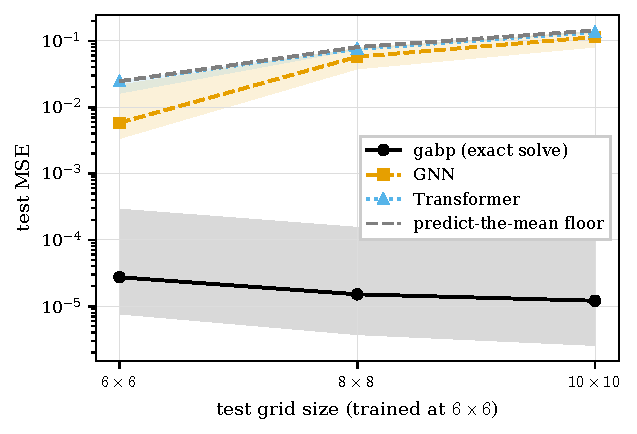
\includegraphics[width=\mazeextrapolationwidth]{figures/maze_extrapolation.pdf}
  \caption{Test error vs.\ grid size. Lines are medians over seeds 0--2, and
  bands span the corresponding minima and maxima. The exact-solve median
  remains below $10^{-4}$; the tested GNN and Transformer approach the
  predict-the-mean baseline. Data:
  \url{paper/attainability/figures/data/maze_extrapolation.csv}.}
  \label{fig:maze}
\end{figure}
\FloatBarrier

\paragraph{Within-architecture control: the effect is the solve's globality, not the
architecture.}
The much larger baselines show that the observed gap is not explained by raw
trainable-parameter count alone, but they differ in architecture and
optimization, so the gap could still be architectural. To isolate the
computation, the within-architecture intervention holds the \texttt{gabp}
model identical (same encoder, same
parameter count, same data and optimizer) and replaces its exact
\texttt{junction\_solve} with $K$ damped-Jacobi sweeps on the same learned
precision $A$. Starting from zero, each sweep expands point-source support by
at most one graph edge; after $K$ sweeps the sharp bound is $K-1$ edges. For
the convergent splitting used here, $K\to\infty$ recovers the exact solve; the
intervened variable is the iteration budget. The error decreases monotonically
with that budget
(Table~\ref{tab:maze-causal}, Figure~\ref{fig:maze-causal}): every displayed
finite-budget variant is worse than predict-the-mean (a truncated solve yields
a confidently wrong near-source field), and only the exact, global solve is
below that baseline. Its error is more than three orders of magnitude below
the deepest truncation. A matched-fit check on the held-out seeds (below)
shows why: the
preregistered $K=7$ arm cannot reach the exact arm's \emph{training} fit
(median relative train-loss gap $\sim2000\times$), so this
dose-response is best read as an attainability/optimization gap: the
finite truncations tested do not reproduce the globally coupled target.
It is not evidence that exactness biases training toward a
better solution among equally attainable ones.

\begin{table}[htbp]
  \centering
  \caption{Within-architecture Jacobi-budget control at $6\times6$; only the solve
  changes. Central processing unit (CPU), 64-bit floating-point (fp64), seed
  0. Displayed values are rounded conservatively
  against the exact-solve arm. Data:
  \url{paper/attainability/figures/data/maze_causal.csv}.}
  \label{tab:maze-causal}
  \begin{tabular}{lccccccc}
    \toprule
    Jacobi sweeps $K$ & 1 & 2 & 4 & 8 & 16 & 32 & exact \\
    \midrule
    test MSE & $2.9\mathrm{e}{-1}$ & $2.5\mathrm{e}{-1}$ & $2.1\mathrm{e}{-1}$ & $1.6\mathrm{e}{-1}$ & $1.0\mathrm{e}{-1}$ & $5.2\mathrm{e}{-2}$ & $\mathbf{1.2\mathrm{e}{-5}}$ \\
    \bottomrule
  \end{tabular}
\end{table}

\providecommand{\mazecausalwidth}{0.72\textwidth}
\begin{figure}[htbp]
  \centering
  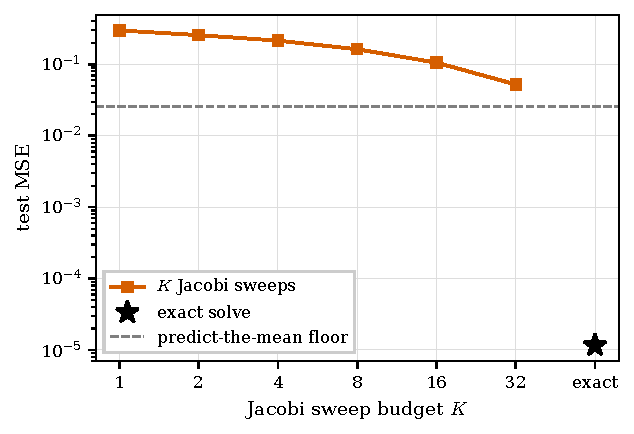
\includegraphics[width=\mazecausalwidth]{figures/maze_causal.pdf}
  \caption{Within-architecture Jacobi-budget control. Test error decreases with
  Jacobi depth $K$, but the finite variants do not attain the exact arm's
  training fit. Data:
  \url{paper/attainability/figures/data/maze_causal.csv}.}
  \label{fig:maze-causal}
\end{figure}

\paragraph{Preregistered matched-fit result on held-out seeds.}
The confirmatory test ran the routed-field task at sizes $6\times6$ to
$48\times48$ on $30$ reserved held-out seeds ($1000$--$1029$), comparing the
exact solve against a compute-matched truncated (Jacobi) baseline within the
same model class, under matched-fit decision rules frozen before the run
(thresholds predeclared in
\url{archive/docs/PREREGISTRATION_MATCHED_FIT_CONFIRMATORY.md}; the
confirmatory gates and per-cell adjudication are recorded in
\url{archive/docs/CONFIRMATORY_RESULTS.md}). The preselected $K=7$ arm is
\textbf{unmatchable for all $30$ seeds}: median exact training loss
$1.45\times10^{-5}$ against that arm's best of $2.96\times10^{-2}$,
a relative gap of about $2000\times$. Thus no matched-fit regime exists for
the confirmatory arm, supporting an attainability reading rather than a
preference among equally fit models. The
as-trained gap also shrinks with size ($8.17\times10^{-2}$ at size $6$ to
$1.30\times10^{-3}$ at size $48$), so there is no growing-extrapolation
signal beyond the attainability gap itself.
\providecommand{\tmlrevidencestart}{}
\providecommand{\tmlrevidenceend}{}
\tmlrevidencestart
Full verdict and per-seed records:
\url{archive/docs/CONFIRMATORY_RESULTS.md} (Maze section),
\url{archive/results/CONFIRMATORY/matched_fit_taskA/maze_matched_fit.json},
and \url{archive/results/CONFIRMATORY/matched_fit_taskA/maze_seeds/}.
\tmlrevidenceend
The $K=256$ floor arm's mean absolute extrapolation gaps are 3.8--4.6 orders
below the $K=7$ gaps, which is the comparison the frozen results prose used to mark
maze NC2 as passing. However, the same first-read JSON records
\texttt{floor\_sound=false}: at size 6, the mean floor-minus-exact loss gap is
$2.70\times10^{-5}$, or $44\%$ of the exact arm's mean evaluation loss,
against the implementation's separate $5\%$ in-distribution diagnostic.
Because the preregistration says ``function/extrapolation distance'' without
resolving these two checks, the manuscript treats the maze near-exact control
(NC2) as ambiguous, not as a clean pass.

\paragraph{Interpretation and scope.}
The task is solve-shaped by construction: the label is the output of a
structured global solve, and the \texttt{gabp} model contains that operator.
This accounts for the observed advantage over the tested GNN and Transformer
baselines. The preregistered matched-fit evidence does not establish
the stronger inductive-bias reading: that among models capable of comparably
fitting the training data, embedding the exact solve is what tips training
toward the generalizing one. The bounded-reach and message-passing
alternatives here are not comparably capable at these budgets; they do not
fit the target in the hard regime, which is an attainability/optimization
gap, not evidence of an implicit training preference.
Section~\ref{sec:program} states the benchmark-scale version and what would
falsify or refine this reading.

\section{Probe 2: stiff-regime training with exact implicit gradients}
\label{sec:deq}

The second axis is stability. A model's optimum can lie where the underlying
fixed point is stiff: long memory, strong coupling, slow mixing. Finite
unaccelerated gradient estimates can become inaccurate there. This section
shows that the exact selected-inverse backward keeps gradients correct in the
tested regime, so it can train where the tested finite Neumann adjoints do not.

\paragraph{The operator's role.}
A deep-equilibrium layer defines its output as a fixed point
$z^\star = f(z^\star, x)$. The implicit function theorem makes its backward
pass a single non-symmetric solve with the equilibrium Jacobian
$J=\partial f/\partial z$,
\begin{equation}
  (I-J)\T u = \partial\loss/\partial z^\star,
  \qquad \partial\loss/\partial\theta = u\T \,\partial f/\partial\theta .
  \label{eq:ift}
\end{equation}
When the coupling of $f$ is sparse on a low-treewidth graph, which is this
paper's regime, \eqref{eq:ift} is exactly the non-symmetric junction solve
sibling of selected inversion on $A = I-J$: one block $LDU$ factorization at
$\Theta(Wb^3)$ structural work,
with the transposed factor roles giving the adjoint without a second factorization
(Remark~\ref{rem:scaffold}). Common DEQ implementations obtain the adjoint
iteratively; the transparent baseline here uses
$u_{k+1} = J\T u_k + g$. After $K$ terms, the
Neumann tail is $(J\T)^K u^\star$; its asymptotic rate is governed by
$\rho(J)$, with constants and transients affected by non-normality. Thus the
unaccelerated iteration can become arbitrarily slow as $\rho(J)\to1$.

\paragraph{Result on four tested $\rho$ values: sparse direct remains accurate; finite
Neumann truncations degrade.}
On a non-symmetric coupling on a loopy $3\times3$ grid (genuine fill) scaled
to a target spectral radius, the experiment measures the parameter-gradient relative error
against a dense implicit-differentiation oracle (Table~\ref{tab:deq},
Figure~\ref{fig:deq}). The sparse-direct backward stays within
$1.1\times10^{-12}$ of the dense fp64 oracle on these four cells. Its error
rises as the system becomes nearly singular, as ordinary condition-sensitive
direct-solve analysis predicts. The iterative
backward degrades with the Neumann tail: at $\rho=0.99$ even $32$ terms leave
relative gradient error $77.1\%$, and at $\rho=0.999$ the error is $97.4\%$.
Separate unit tests validate the nonlinear implicit-function-theorem
backward against autograd through an unrolled solver
(\url{tests/test_deq_fixedpoint.py}).

\begin{table}[htbp]
  \centering
  \caption{Parameter-gradient relative error against a dense
  implicit-differentiation oracle as $\rho(J)\to1$. One deterministic instance
  per spectral radius, seed 0; central processing unit (CPU), 64-bit
  floating-point (fp64). Displayed values are rounded
  conservatively against sparse direct. Data:
  \url{paper/attainability/figures/data/deq_robustness.csv}.}
  \label{tab:deq}
  \begin{tabular}{rcccc}
    \toprule
    $\rho(J)$ & sparse direct & Neumann-8 & Neumann-16 & Neumann-32 \\
    \midrule
    $0.500$ & $\mathbf{1.83\mathrm{e}{-16}}$ & $1.17\mathrm{e}{-2}$ & $4.99\mathrm{e}{-5}$ & $7.55\mathrm{e}{-10}$ \\
    $0.900$ & $\mathbf{5.15\mathrm{e}{-16}}$ & $6.69\mathrm{e}{-1}$ & $3.05\mathrm{e}{-1}$ & $5.63\mathrm{e}{-2}$ \\
    $0.990$ & $\mathbf{1.65\mathrm{e}{-14}}$ & $9.74\mathrm{e}{-1}$ & $9.06\mathrm{e}{-1}$ & $7.71\mathrm{e}{-1}$ \\
    $0.999$ & $\mathbf{1.08\mathrm{e}{-12}}$ & $9.97\mathrm{e}{-1}$ & $9.90\mathrm{e}{-1}$ & $9.74\mathrm{e}{-1}$ \\
    \bottomrule
  \end{tabular}
\end{table}

\begin{figure}[t]
  \centering
  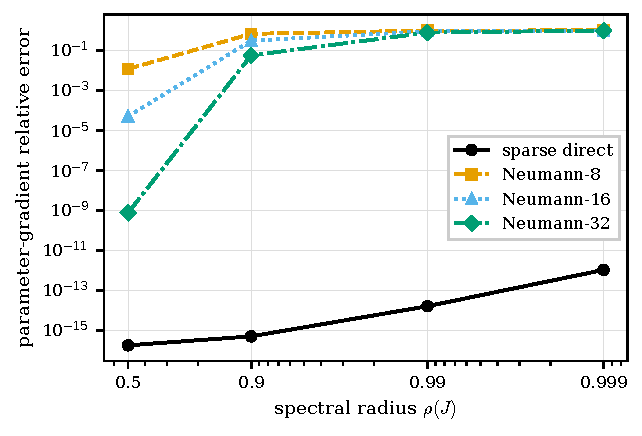
\includegraphics[width=0.72\textwidth]{figures/deq_robustness.pdf}
  \caption{Implicit-gradient error for sparse direct and finite Neumann
  adjoints. One deterministic instance is shown at each spectral radius;
  this is a finite diagnostic, not a
  condition-independent stability claim. Data:
  \url{paper/attainability/figures/data/deq_robustness.csv}.}
  \label{fig:deq}
\end{figure}

\paragraph{Confirmatory training-level test on held-out seeds.}
The gradient-error measurement above is exploratory, so a confirmatory,
training-level version of the claim was preregistered and run once on $30$
reserved held-out seeds ($1000$--$1029$) on their first aggregate read. Both
arms train a scalar gain through the same exact forward
solve ($n=16$, non-symmetric coupling), held bit-identical between arms; the
only intervention is the backward rule used during training, the exact
implicit adjoint versus a biased $K$-term Neumann adjoint. The
preregistered matched-fit adjudication
(\url{archive/bench/matched_fit_taskA.py}) distinguishes an equal-fit
preference from attainability by checking whether the Neumann arm can match the
exact arm's training loss (gated by a frozen floor and a $60\%$ matchability
bar) before crediting any test-loss gap to an inductive-bias mechanism. In
the stiff cells ($\rho\in\{0.98,0.99\}$ and $K\in\{1,2,4\}$) the
Neumann arm is matchable in only $0$--$23.3\%$ of seeds
(relative train gap $+1.45$ to $+13.2$), so the inductive-bias
(\textsc{survive}) branch has nothing to compare there; the result resolves to
the conservative attainability/optimization reading. That branch is also
unreachable at the one high-$\rho$ arm that does clear the matchability bar,
because that arm calibrates the floor it would have to exceed; this is a
defect of the frozen rule rather than a finding, and
Appendix~\ref{app:integrity} states it. The one designed silent
control ($\rho=0.5$) did not cleanly pass: its relative-gap clause failed
(driven by a denominator-scale instability in the relative ratio, with both arms
converging to losses of order $10^{-8}$--$10^{-9}$), though its
independent function-distance clause passed by more than four orders of
magnitude. Per the frozen rule (a positive reading is void unless its
negative controls hold), this is reported as a hedged, not pristine,
conservative verdict, not relaxed after the fact. Full adjudication, per-cell
table, and per-seed records:
\url{archive/docs/CONFIRMATORY_RESULTS.md},
\url{archive/docs/PREREGISTRATION_MATCHED_FIT_CONFIRMATORY.md}, and
\url{archive/results/CONFIRMATORY/matched_fit_taskA/deq_matched_fit.json}.

A later branch reused the same HOLDOUT seeds for a different bootstrap
analysis after this first read. That second use is not an independent
confirmation, and none of its verdicts or effect-size claims is used here.
Appendix~\ref{app:integrity} records the chronology and a nested run-tag
metadata defect.

\paragraph{Interpretation and scope.}
The error sweep is a mechanism result at controlled scale ($n=9$): it shows
the exact sparse-direct backward is accurate on the tested cells where the
finite Neumann truncation is not, and that the training arms differ in
attainability under the first-read protocol. The adjudication does not support
the stronger claim that this difference reflects an inductive bias among
equally attainable optima, because the hard cells do not supply an equal-fit
comparison. On this evidence, the observed difference reflects the iterative
arm's inability to fit the stiff cells, an attainability/optimization effect
rather than a preference effect. Neumann iteration is the transparent
baseline; accelerated solvers (Anderson \citep{anderson1965iterative} and
Broyden \citep{broyden1965class}) can reduce the iteration count and are
necessary competitors at scale; they were not evaluated here. The structured
direct solve avoids a convergence tolerance but retains ordinary
conditioning-dependent rounding error. The affine diagnostic uses a
convergent construction with $\rho(J)<1$; the advantage is for
graph-structured, low-treewidth Jacobians. For a dense $J$, the $LDU$
factorization is $\bigO(n^3)$ and an
iterative method may be preferable. A benchmark-scale learned-capability gain
has not been demonstrated and would need its own matched-fit or attainability
control for a valid attribution.

\section{A falsifiable program: where exactness should and should not help}
\label{sec:program}

The two probes at controlled scale (Sections~\ref{sec:maze}
and~\ref{sec:deq}) resolved to attainability, not inductive bias: the
pre-registered matched-fit design found the exact solve wins because the
alternatives cannot fit the task, not because it tips training toward a
better solution among equally-attainable ones. What survives is the
operator's classical, verified numerical properties -- exact, deterministic,
$\bigO(\text{fill})$ -- against incumbents that are stochastic, iterative, or
conditioning-dependent. This section states that operator gap, the
benchmark-scale experiments that would show it matters (or does not), the
negative control, and the single prerequisite that gates all of them. None of
what follows claims inductive bias; each hypothesis below is a numerical or
capability claim, stated so it can be wrong.

\paragraph{The operator gap (what scalable differentiable-sparse methods must match).}
Three capabilities anchor the claim; each is exact and deterministic where the
incumbents are stochastic, iterative, or conditioning-dependent.
\begin{itemize}
  \item \textbf{M1: exact, deterministic} gradient of $\log\det A$ and exact
        on-pattern blocks and diagonal of $\inv{A}$, at $\bigO(\text{fill})$.
        Incumbent: the conjugate-gradient plus stochastic-Lanczos-quadrature
        gradient of GPyTorch \cite{gardner2018gpytorch,ubaru2017fast} is
        variance-laden and $\kappa$-biased, with no exact $\diagop(\inv{A})$
        at scale.
  \item \textbf{M2: conditioning-independent, constant-memory adjoint.} A
        direct factorization gives an $\bigO(\text{fill})$-memory,
        iteration-free adjoint whose accuracy does not degrade with $\kappa$
        or $\rho(J)$ (Section~\ref{sec:deq}). Incumbents: unrolled iterative
        adjoints store $\bigO(K)$ states; implicit CG and AMG adjoints
        reintroduce $\kappa$-dependent iteration and gradient bias.
  \item \textbf{M3: a one-layer, exact, differentiable global graph
        functional} (resolvent, effective resistance, commute time), where
        bounded-depth message passing provably needs $\Omega(\text{diameter})$
        depth and transformers approximate without extrapolating
        (Section~\ref{sec:maze}).
\end{itemize}

\paragraph{Benchmark-scale experiments.}
Each attacks one capability on real, non-toy data, with a falsification bar
that should be fixed before the benchmark is run.
\begin{itemize}
  \item \textbf{E2 (M1): exact deterministic gradients for calibrated UQ.}
        Hypothesis: exact marginal-likelihood gradients and exact posterior
        marginal variances give better-calibrated uncertainty and more stable
        hyperparameter optimization than CG plus SLQ, with the gap widening as
        the noise tends to zero and $\kappa$ grows. Competitors: GPyTorch
        \cite{gardner2018gpytorch}, SKI/KISS-GP \cite{wilson2015kernel},
        Vecchia approximations \cite{katzfuss2021general}, and SVGP
        \cite{hensman2013gaussian}. Data: ERA5/NOAA spatial GMRFs and PeMS
        state-space GPs. \emph{Falsified if} SLQ/CG gradients are within noise
        of exact on real data at feasible cost.
  \item \textbf{E1 (M2): constant-memory, conditioning-independent adjoints
        for differentiable physics.} Hypothesis: on high-contrast 2-D
        PDE-constrained learning, the exact sparse-direct adjoint gives
        gradients whose error and backward memory are flat in the condition
        number, where unrolled CG runs out of memory and implicit AMG adjoints
        stall or bias. Competitors: unrolled CG and implicit CG/AMG adjoints.
        Data: high-contrast Darcy flow on SPE10 permeability (contrast up to
        $10^7$); a sparse-observation inverse problem. \emph{Falsified if}
        AMG-preconditioned implicit adjoints stay accurate and cheap at $10^7$
        contrast.
  \item \textbf{E3 (M3): the exact resolvent layer vs.\ over-squashing and
        size extrapolation.} Hypothesis: one exact differentiable resolvent
        layer computes global functionals that bounded-depth message passing
        cannot, removing over-squashing
        \cite{alon2021bottleneck,topping2022understanding} and generalizing
        across graph sizes where GNNs, rewiring, and graph transformers
        degrade. This is the benchmark-scale version of
        Section~\ref{sec:maze}. Competitors: strong MPNNs, graph rewiring
        (SDRF \cite{topping2022understanding}, FoSR \cite{karhadkar2023fosr}),
        graph transformers (GPS \cite{rampasek2022recipe}, Exphormer
        \cite{shirzad2023exphormer}), and implicit GNNs \cite{gu2020implicit}.
        Data: the Long Range Graph Benchmark \cite{dwivedi2022long} and real
        road networks with train-small/test-large splits. \emph{Falsified if}
        a graph transformer matches both in distribution and across the
        extrapolation sweep.
  \item \textbf{E4 (M2, deepest): training at the edge of stability.} The
        benchmark-scale version of Section~\ref{sec:deq}: does the exact
        backward let one train structured equilibrium models at near-critical
        $\rho(J)\to1$, a regime that phantom-gradient \cite{geng2021training}
        and Anderson/Broyden adjoints
        \cite{anderson1965iterative,broyden1965class} cannot reach, for a
        learned-capability gain (longer effective range)? \emph{Falsified if} phantom-gradient
        DEQs train fine without ever needing high $\rho$, i.e.\ the useful
        regime is not stiff.
\end{itemize}

\paragraph{The negative control.}
Every generalization experiment includes a task \emph{not} reducible to a
structured global solve, where any exactness-specific explanation,
attainability included, predicts the advantage
must vanish. A persistent gap there would mean the effect is a confound
(capacity, optimization, data leakage), not exactness; its absence is what
supports the attribution reading of Section~\ref{sec:maze} at scale.

Two pre-registered negative controls have already been run at small scale,
and neither passed cleanly, which is exactly why Sections~\ref{sec:maze}
and~\ref{sec:deq} resolve to the conservative attainability reading rather
than a confirmed inductive bias. On the maze held-out seeds, a
short-correlation-length variant of the routing task ($\varepsilon=2.0$,
where the solve's reach should barely matter) still showed the exact solve
beating the compute-matched truncation at every size -- a disclosed limitation
of the matched-compute cost story. On the DEQ held-out seeds, the low-$\rho$
silent control's relative-gap clause failed at near-machine-precision loss
levels, though its independent function-distance clause held by more than
four orders of magnitude (Section~\ref{sec:deq}). Per the frozen rule, a
failed negative control voids a clean positive reading; neither probe gets
one. The benchmark-scale negative controls above carry the same commitment:
if they fail, the failure is reported, and a future benchmark-scale
inductive-bias test would need a cleaner control (keyed on function distance,
not relative gap, at near-machine-precision cells) before it could confirm
anything.

\paragraph{The one prerequisite, and the one falsification that sinks it.}
All of the above need problems larger than today's per-node Python-loop CPU
ceiling. The gating item is a single, already-scoped engineering build, a
GPU-batched junction kernel, not new theory; until it runs, the claim is
established only at the controlled scale of Sections~\ref{sec:maze}
and~\ref{sec:deq}. One outcome would bound the whole program: if real
low-treewidth problems are mostly well-conditioned (where iterative and
stochastic gradients are good enough) and real stiff problems are mostly dense
3-D (multigrid territory), then the operator gap lands where it is not needed.
E1 and E2 are designed so that their failure pins down that
boundary, in which case the result is a characterization of where exactness
matters.

\section{Related work}
\label{sec:related}

\paragraph{The exact engine.}
The Takahashi equations \citep{takahashi1973} and Erisman--Tinney
\citep{erismantinney1975} compute inverse entries on the Cholesky factor's
pattern without the full inverse; SelInv \citep{lin2011selinv} and the pole
expansion and selected inversion method (PEXSI)
\citep{lin2013pexsi} do this for general sparse SPD and Hermitian matrices via
the elimination tree, and \citet{jacquelin2018pselinv} carry the same
distributed algorithm to non-symmetric $A$ with the selection confined by the
pattern of $A\T$; Gaussian belief propagation is the same
collect/distribute recurrence and is exact on trees
\citep{weiss2001correctness,bickson2008gaussian}. Recent accelerator systems
include \texttt{Serinv} for block-tridiagonal arrowhead matrices
\citep{maillou2025serinv} and tile-parallel selected inversion for structured
matrices \citep{fattah2025stiles}. This work is a reference PyTorch
implementation, not a performance competitor to those systems, and claims
nothing new for the forward recurrence.

\paragraph{Differentiating selected inversion.}
The reverse-mode adjoint of the matrix inverse,
$\cotan{A}=-\inv{A}\cotan{G}\inv{A}$, is folklore
\citep{dwyer1948symbolic,giles2008collected}; that its evaluation costs a
constant factor of the forward is the cheap-gradient principle
\citep{baur1983complexity}. \citet{zhu2019sparse} differentiate a sparse
log-determinant through selected inversion on the same factorization; this is
standard in GMRF and sparse-Cholesky learning \citep{rue2005gmrf}. Template
Model Builder (TMB) has
long combined sparse latent-Gaussian calculations,
automatic differentiation, and Laplace approximation at large scale
\citep{kristensen2016tmb}. These results provide the mathematical background for
Remark~\ref{rem:scaffold}.

\paragraph{Differentiable sparse linear algebra.}
Schwarz--Schur Involution batches direct sparse subdomain operations on GPUs
and supplies a differentiable solver for PDE-shaped problems
\citep{wang2025schwarz}. \texttt{torch-sla} unifies differentiable direct,
iterative, nonlinear, and eigenvalue solvers across CPU, GPU, and distributed
backends \citep{torchsla2026}. Closest to the operator surface here,
\citet{boudaoud2026adelia} register a hand-derived \texttt{custom\_vjp} in JAX
covering factorization, triangular solve, and selected inversion, for the INLA
objective on symmetric block-tridiagonal arrowhead precision matrices. These
systems make a generic ``differentiable sparse solver'' claim untenable, and a
differentiable selected inverse is not by itself unoccupied. The narrower
software surface here is selected covariance entries, log determinant, solve,
and sampling on a general filled pattern, exposed as a trainable PyTorch layer
and including a static-pattern non-symmetric selected inverse rather than a
symmetric inference backend. The
paper's scientific contribution is
instead the preregistered account
(Sections~\ref{sec:maze}--\ref{sec:deq}) of why exactness wins on its
solve-shaped probes: attainability against bounded-reach or biased-gradient
alternatives, not an inductive-bias effect. Approximate selected-covariance
methods with estimable confidence bounds \citep{siden2017covariance} are
important competitors for the prospective uncertainty experiment.

\paragraph{Where the claim lives.}
The original motivation drew on the lineage of inductive bias for
generalization and size or length extrapolation; the evidence in this paper
instead lands on the expressivity limits of bounded-depth message passing,
including the over-squashing line
\citep{alon2021bottleneck,topping2022understanding}
and graph rewiring \citep{topping2022understanding,karhadkar2023fosr},
implicit and steady-state graph neural networks \citep{gu2020implicit}, and
graph transformers \citep{rampasek2022recipe,shirzad2023exphormer}. Since the
matched-fit result says the tested alternatives do not attain the target, the
evidence supports an
expressivity/attainability story rather than a generalization-preference
one. These methods are the relevant comparator set for any future
expressivity-separation claim. The consumers
that make a differentiable selected inverse useful, deep equilibrium models
\citep{bai2019deep} and delta-rule linear-attention layers
\citep{yang2024parallelizing}, supply the structured symmetric and
non-symmetric solves of Section~\ref{sec:deq} and the appendix. That
literature also argues the other way: Jacobian-free backpropagation drops the
Jacobian term outright and reports accuracy competitive with prior implicit
networks at matched parameter count \citep{fung2022jfb}, and phantom gradients
report an inexact update direction that is empirically preferable
\citep{geng2021training}. Neither estimator is a fixed-$K$ Neumann truncation
and neither is evaluated with $\rho(J)$ near one, which is where
Section~\ref{sec:deq} places its hard cells. The attainability reading is
scoped to that estimator in that regime, not to inexact implicit gradients in
general.

\section{Conclusion}
\label{sec:conclusion}

The selected inverse is a classical, exact, $\bigO(\text{fill})$ global operator, and,
because it is the gradient of a log-determinant, it is cheap to
differentiate. Those facts are not new, and this paper's own numerics rule
out the obvious payoff: exactness buys nothing on the precision axis
(Section~\ref{sec:numerics}). The hypothesis under test was that it buys
something else instead -- that exactness is an inductive bias, changing which
of two equally-fit models is preferred. Two pre-registered, matched-fit
probes on $30$ held-out seeds test this directly, and on both, the
inductive-bias branch does not fire: the alternative (bounded-reach sweeps in
Section~\ref{sec:maze}, the biased Neumann adjoint in Section~\ref{sec:deq})
cannot reach comparable training fit at the difficulty levels where the raw
gap is largest, so the gap is explained by attainability, not by an implicit
preference among optima that fit equally well. This is a real finding, not a
null one: it says the practical advantage of embedding the exact solve --
still a factor of roughly $600\times$ to $28{,}000\times$ across the tested
sizes -- comes from
the alternatives' inability to represent or optimize the target, not from a
training-time bias effect. Both probes' negative controls are disclosed as
imperfect (Section~\ref{sec:program}), so even this conservative reading is
reported as hedged, following the frozen pre-registration rather than
relaxing it post hoc.

The limits are explicit: the evidence is at controlled CPU scale and
confined to low-treewidth (1-D and quasi-2-D) problems. What remains open is
whether exactness matters for reasons unrelated to inductive bias: exact
deterministic gradients for calibrated uncertainty quantification,
conditioning-independent adjoints for differentiable physics, and a
one-layer exact resolvent against message-passing's bounded-depth limits
(Section~\ref{sec:program}). These are numerical and expressivity claims,
each with its own falsification bar, gated on a single scoped build: a
GPU-batched kernel. The next step is to run them. If they confirm the claim,
exactness's numerical properties become a design principle for
solve-shaped learning at scale; if they fail, they pin down where exactness
does not matter, which is itself an answer. What this paper does not
support, on its own pre-registered evidence, is the inductive-bias framing
that motivated it.


\section*{Acknowledgements}
I thank Isaac Liao (Carnegie Mellon University) for informal technical
discussions that identified selected inversion as a useful operator family,
emphasized the high-condition well-scaled regime and dense-reference precision
comparisons, and suggested a maze-style attribution test.

\appendix
\section{The tree selected-inverse schedule and its projected adjoint}
\label{app:theorem}

This appendix states the classical machinery used in
Section~\ref{sec:theorem}: the tree recurrence that makes the layer exact and
global, and the projected-Hessian argument for its first-order adjoint.

\subsection{Forward: a two-pass schedule on the elimination tree}

\begin{theorem}[Tree selected inverse]
\label{thm:tree-forward}
Let $\Gr$ be a tree rooted at $r$ and $A$ SPD with pattern $\Gr$. Order nodes
so that each precedes its parent. Then \textbf{(a) zero fill:} the block
$LDL\T$ factorization in this order has $L$ unit lower-triangular with the
pattern of $A$ and every pivot $\piv{v}$ SPD; \textbf{(b) collect
(leaves$\to$root):}
$\piv{v} = \Ablock{v}{v} - \sum_{c\in\children(v)} \Ablock{v}{c}\inv{\piv{c}}\Ablock{c}{v}$
and $\Gblock{r}{r} = \inv{\piv{r}}$; \textbf{(c) distribute
(root$\to$leaves):} with $\fac{v} = \Ablock{\parent(v)}{v}\inv{\piv{v}}$,
\[
  \Gblock{\parent(v)}{v} = -\,\Gblock{\parent(v)}{\parent(v)}\,\fac{v},
  \qquad
  \Gblock{v}{v} = \inv{\piv{v}} + \fac{v}\T \Gblock{\parent(v)}{\parent(v)} \fac{v}.
\]
This produces every block of $\selinv(A)$ exactly in
$\bigO((|V|+|E|)\,b^3)$ time and $\bigO((|V|+|E|)\,b^2)$ memory. Steps
(b)--(c) are the tree specialization of the classical Gaussian-BP
collect/distribute and Takahashi recurrences
\citep{weiss2001correctness,takahashi1973}.
\end{theorem}

\subsection{Why the derivative has a same-pattern reverse schedule}

\begin{theorem}[Projected selected-inverse derivative is self-adjoint]
\label{thm:p0}
On the SPD cone, under the full Frobenius inner product on symmetric
matrices, $\selinv_{\pat}(A) = P_{\pat}\nabla_A \log\det A$.
Consequently the Fr\'echet derivative
$D\,\selinv|_A = P_{\pat}\,L_A\,\iota_{\pat}$ (with
$L_A: X\mapsto -\inv{A}X\inv{A}$ the derivative of inversion and $P_{\pat}$
the on-pattern projection, and $\iota_{\pat}$ the inclusion of symmetric
on-pattern perturbations) is self-adjoint: it is the projected Hessian of a
scalar potential, and a gradient field has a symmetric Jacobian (symmetry of
second derivatives).
Hence, for the tree schedule above, the reverse-mode map
$\cotan{G}\mapsto\cotan{A}$ equals the forward derivative map and is realized
by reversing the schedule of Theorem~\ref{thm:tree-forward} at the same structural work
(cheap-gradient principle \citep{baur1983complexity}).
\end{theorem}

\begin{remark}[Self-adjoint up to transpose; the non-symmetric correction]
\label{rem:transpose}
For non-symmetric $A$,
$L_A^* : X\mapsto -A^{-\mathsf{T}}XA^{-\mathsf{T}} = L_{A\T}$, so the adjoint
is $P_{\pat}L_{A\T}\iota_{\pat}$: the projected inversion derivative
evaluated at $A\T$. It is not itself the selected inverse of $A\T$. The
non-symmetric (LU / Erisman--Tinney) kernels are therefore not literally
self-adjoint; the derivative is adjoint up to transpose, which is why
their backward propagates independent lower and upper factor cotangents (the
$L$ of $A$ is the $U$ of $A\T$).
\end{remark}

\begin{remark}[Why the naive off-pattern argument fails]
It is tempting to argue that $\cotan{A}|_{\pat}$ never references an
off-pattern block of $\inv{A}$. That is false:
$\cotan{A}_{vv} = -\sum_{(s,t)\in\pat} \Gblock{v}{s}\cotan{G}_{st}\Gblock{t}{v}$
involves off-pattern $\Gblock{v}{s}$. What is true is that the reverse
schedule never forms them: it propagates cotangents along tree edges, exactly
as the forward computes $\Gblock{v}{v}$ without forming the dense inverse.
The first-order reverse schedule closes on the pattern. This statement alone
does not establish pattern closure or the cost of arbitrary higher-order
derivatives.
\end{remark}

\section{Engine details: generality, stability boundary, and a drop-in}
\label{app:engine}

\paragraph{No-pivot stability boundary (non-symmetric).}
The non-symmetric kernels eliminate on a static pattern with no pivoting,
valid while pivots stay non-singular.
On the tested sweep this is at parity with a pivoted dense LU while the
system is block-diagonally dominant, with the accuracy floor collapsing below the
dominance boundary. The SPD experiment shows a small reconstructed-factor
residual on the finite tree/conditioning grid tested; it does not prove a
height- or $\kappa$-independent global backward-error theorem. The
non-symmetric diagnostic additionally exposes the no-pivot boundary. These
are numerical-analysis observations with no demonstrated learning payoff,
which is why they are not in the body. Data:
\href{paper/attainability/figures/data/nonsym_stability.csv}
{\texttt{nonsym\_stability.csv}} and
\href{paper/attainability/figures/data/stability.csv}
{\texttt{stability.csv}}; generator:
\href{paper/attainability/make_figures.py}{\texttt{make\_figures.py}}.

\paragraph{DeltaNet chunk inverse (a drop-in capability note).}
The differentiable triangular chunk inverse $(I-A)^{-1}$ drops, unchanged,
into a chunked delta-rule linear-attention layer
\citep{yang2024parallelizing}: the within-chunk delta rule \emph{is} that
triangular solve. It reproduces the token-by-token delta rule exactly, and
its analytic backward equals autograd through the whole multi-chunk layer.
Because the forward is identical by construction, this demonstrates
availability (the operator is a genuine drop-in), not a capability gain, and
so it is recorded here rather than as a result. A learned-capability payoff for
sequence models would be a learned-sparse graph-coupled mixer, which belongs
to the program of Section~\ref{sec:program} rather than to the present
evidence.

\section{Confirmatory evidence chronology}
\label{app:integrity}

At repository commit \evidencecommit{}, the matched-fit protocol was frozen
on 29 June 2026, before the first aggregate read of HOLDOUT seeds 1000--1029.
The evidentiary records are \url{archive/docs/CONFIRMATORY_RESULTS.md} and
\url{archive/results/CONFIRMATORY/matched_fit_taskA/}; only these support the
paper's confirmatory interpretation.

On 30 June, a later branch froze a bootstrap protocol and reused the same
HOLDOUT seeds. Its assertion that the seeds were untouched is false in
wall-clock chronology, so that use is not an independent confirmation and
its verdict and effect-size claims are excluded. Both protocol files retain
dated provenance notes.

The first-read \texttt{summary.json} records a top-level
\texttt{run\_tag=CONFIRMATORY}, the HOLDOUT seed list, and a confirmatory
output path, but two nested payloads say \texttt{EXPLORATORY}. In
\url{archive/bench/matched_fit_taskA.py}, those labels come from a module-level
constant; seed guarding and output routing use the confirmatory function
argument. This metadata defect does not change a metric and remains disclosed
in the frozen record.

The maze summary contains a second ambiguity. Its \texttt{floor\_sound} field
is \texttt{false}: at the in-distribution size, the $K=256$ floor arm's mean
evaluation-loss gap from exact is $2.70\times10^{-5}$, versus the
implementation's $3.07\times10^{-6}$ threshold. Results prose nevertheless
marked maze NC2 as passing because its mean absolute extrapolation gaps were
3.8--4.6 orders below the $K=7$ gaps, the narrower check implemented by
\texttt{confirmatory\_decision}. The preregistration required collapse in
``function/extrapolation distance'' and did not specify which of these
non-equivalent summaries controlled. This manuscript does not retroactively
choose the favorable one: maze NC2 is ambiguous, and no positive conclusion
depends on treating it as a pass.

A third defect is structural and was found in a 2026-07-25 re-audit of the
frozen adjudication code. The preregistration defines
$F=\max(2M_{\mathrm{null}},2\times10^{-6})$, where
$M_{\mathrm{null}}$ is the near-exact cell's own matched function distance,
and applies $F$ to both that cell's C2 collapse test and the rival
inductive-bias branch. At high difficulty, $K=32$ is the only arm reaching
the $60\%$ matchability bar and thus the only adjudicable equal-fit arm; it
also sets $M_{\mathrm{null}}$, so its distance is compared with twice itself.
In
\url{archive/bench/matched_fit_taskA.py}, the verdict is \textsc{survive} when
the matched distance's confidence interval (CI) lower bound exceeds $F$,
\textsc{collapse} when its mean is at most $F$, and \textsc{ambiguous}
otherwise. With $F=2\times$ that mean, \textsc{collapse} is forced and
\textsc{survive} is unreachable. C2's recorded pass is therefore
uninformative, and the inductive-bias branch could not have fired on these
data regardless of the measurements. Measured instead against the
preregistration's absolute optimization-noise scale $2\times10^{-6}$,
calibrated on development seeds where the largest silent-cell matched distance
was $1.46\times10^{-6}$, the two near-exact distances
($9.11\times10^{-4}$ at $\rho=0.98$ and $1.83\times10^{-4}$ at $\rho=0.99$)
are $455\times$ and $91\times$ larger, and the $\rho=0.98$ CI lower bound
($3.84\times10^{-4}$) also exceeds it. We report the frozen rule unchanged.
Thus, the evidence does not support an inductive-bias reading where the finite
arms cannot fit and leaves it untested where they can.


\small
\bibliographystyle{plain}
\bibliography{refs}

\end{document}
